To find \emph{influential} people from the text in news articles, we define a score corresponding to each person entity in the gazetteer. This score is called the \emph{Influential Person Index (IPI)}. To calculate IPI, we first define a \emph{Document Index (DI)} to measure how each document in the person's associated list of documents affects his influence score. The choice of features for detecting whether a person is influential is motivated by following questions: (a) Are people mentioned frequently in the newspaper \emph{influential}? (b) How to measure frequency of occurrence(s) of a person - article by article or across the complete dataset? (c) Do longer documents talk more about important persons? (d) Is a person discussed in varied contexts (and over multiple topics in news) more influential than one who is consistently talked about in articles belonging to a single topic?  The following discussion describes the features chosen for calculation of DI and IPI of a person,followed by the complete algorithm for detection of influential persons.

\noindent \textbf{Document Index (DI): }
%\label{influential:DI}
The Document Index (DI) of an article in the people gazetteer helps to measure a person's influence score. This is calculated as follows:

%\begin{enumerate}
%\item 
\noindent \textbf{Normalized Document Length (NDL): } 
Document Length is defined as the number of tokens contained in a news article. It is further normalized by dividing with the maximum length of a news article. Thus,  

$$NDL=\dfrac{\text{Document Length}} {\text{Maximum Document Length in the dataset}}$$


%\item[$\bullet$IDF]
%IDF is used as a parameter in the calculation of DI of a news article to give weight to the person entity's occurrence in the complete %dataset. It can be calculated as the number of news articles in which a person entity occurs in the complete dataset. It is %equivalent to the length of document list in the people gazetteer for each person entity.

%\item
\noindent \textbf{ Normalized Person Name Frequency (NPNF): }
Person Name Frequency (PNF) accounts for the number of occurrences of a person's name in the news article. A high value of PNF makes the document more important. It is normalized as follows:

\begin{center}
$NPNF=	1+\log$(PNF)
\end{center}

The important questions that arise when dealing with Person Name Frequency are: (a) \textbf{Coreference resolution} of person names: (for e.g., names ``William Schmittberger",``Captain Williams" are same but recognized as separate persons) and (b) \textbf{Named Entity Disambiguation:} This refers to the occurrence of different persons with similar name in news articles. For e.g., the person ``John Smith" detected in two different articles may or may not refer to the same person. These issues are not dealt with by the PNER and need to be addressed separately. 
%While the issue of coreference can be still addressed by analyzing each news article, it is extremely hard to disambiguate among persons with similar names that can occur in multiple news articles with different topics. This is the reason coreference resolution is performed for the person entities obtained using PNER.
The following section explains the approach to coreference resolution.


\noindent \textbf{Coreference Resolution: } The coreference resolution aims to find all expressions that refer to the same person in the text. 
%Due to multiple references to a person in the text, coreference resolution been done keeping in mind that the number of articles of occurrence of a person entity, i.e.,TF is an important parameter in our study for determining an influential person.
The algorithm used in this work uses a multi-pass sieve for coreference resolution\cite{lee2013deterministic} and consists of three steps: (a) Mention Detection: The goal is to  detect nouns, pronouns and occurrences of named entities from the text (b) Coreference Resolution: This is performed by using a combination of ten independent sieves applied from highest to lowest precision with global information sharing so that each sieve builds on the previously clustered mentions followed by post processing which removes singleton mentions. An implementation of this is available from the Deterministic Coreference Resolution System of the CoreNLP toolkit\footnote{http://nlp.stanford.edu/software/dcoref.shtml}. (c) Identification of the most representative mention: The most representative mention from each coreference chain is found and checked to ensure it is a valid person entity in the People Gazetteer. If it is found, then the count from coreference resolution is considered in the person name frequency determination. 

%% AAYUSHEE PLEASE MODIFY THIS PARAGRAPH
Coreference Resolution was observed to be useful during this case study since the frequency of a person entity in a newspaper article changes when multiple references to the same person entity (coreferences) are found in an article. Figure~\ref{figure:coref}  illustrates an example of coreference resolution when applied to an article text and its effect on term frequency for person entities. Initially, mentions are detected from the text followed by application of coreference resolution step which results in a chain of coference mentions/entities, which includes the mention itself along with other mentions that refer to it. It is also observed that due to lack of punctuation in the dataset, lots of meaningless coreference mentions are also detected. However, since the persons list is available from the People Gazetteer, frequencies of only those person entities are replaced through Coreference Resolution. 
 % ~\ref{figure:core} or
%\begin{figure*}
%\begin{center}
%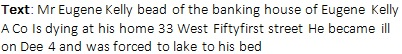
\includegraphics{coref}
%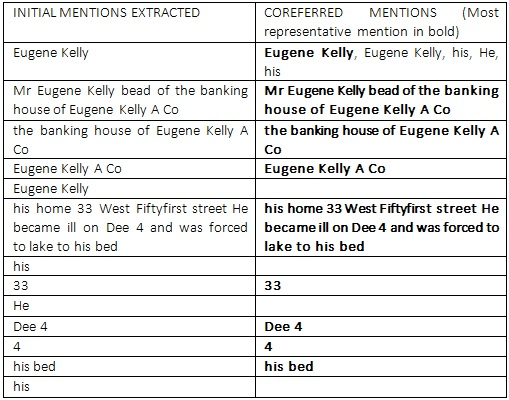
\includegraphics{coref1}
%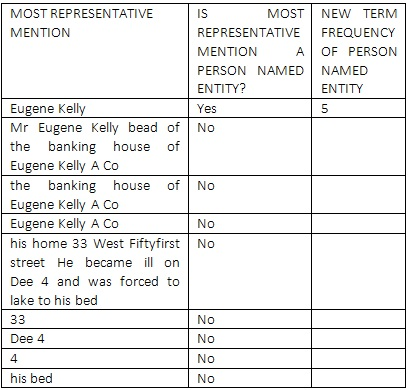
\includegraphics{coref2}
%\end{center}
%\caption{Figure illustrating change in term frequency for person named entities on using coreference resolution on an article text}
%\label{figure:core}
%\end{figure*}

\begin{figure*}
\fbox{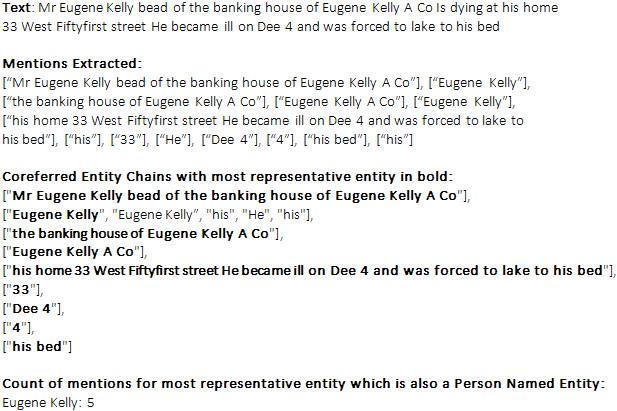
\includegraphics{coref3}}
\caption{Figure illustrating change in term frequency for person named entities on using coreference resolution on an article text}
\label{figure:coref}
\end{figure*}

%\item 
\noindent \textbf{Number of similar articles (NSIM): }
This parameter is used in the calculation of the DI by finding articles belonging the same topic. 
%The set of topics derived from a corpus can be used to answer questions about the similarity of words and 
%documents.
For a document $d$ whose DI is to be calculated, let  SIM= Number of articles with the same topic as $d$ in the document list of a person.
This measure is normalized by the total number of articles in the document list of the person. Formally,

%\begin{center}
$NSIM= \frac{\text{SIM}} {\text{Total number of articles in the person's document list}}$
%\end{center}
NSIM is equivalent to the proportion of topic similar articles that document $d$ has.
%This parameter takes into account the effect of a document's score on a person's IPI when there exist several other documents of the same topic in the person's list. 
%\end{enumerate}
The Document Index is a function of the above mentioned parameters and is calculated by using the following formula:
\begin{center}

			$DI = w_a . NDL + w_b . NSIM + w_c . NTF $
\end{center}
where, $w_a$, $ w_b$ and $w_c$ are the weights for NDL, NSIM and NTF respectively.
DI is a heuristic measure -- each of the parameters can be weighted as per dataset characteristics and user requirements. For example, a higher value to $w_a$ and lower to $w_b$ and $w_c$ indicates documents with longer lengths are considered more important for influencing a person's IPI. On the other hand, a higher value to $w_b$ and lower to $w_a$ and $w_c$ indicates a document with larger proportion of topic similar articles influences the person's IPI more suggesting assignment of high influence score to a person entity occurring repeatedly in a specific news topic.  

\subsection{Influential Person Index (IPI)}

Once DI is calculated, the IPI is estimated as follows:
		
\begin{center}
$IPI= \text{max } DI(d_1, d_2, ...,d_n)+ UniqT$
\end{center}

where, $UniqT = \frac{\text{Number of Unique Article Topics in a person entity's document list}}{\text{Total Number of Topics in the corpus}}$. The parameter $UniqT$  is used to account for the fact that a single person entity can be talked about multiple news topics in the news articles and to include its effect on the person entity's influence score. %It is normalized by dividing it with the total number of topics as obtained during topic detection on all 14020 articles.
To rank people, the IPI are sorted in decreasing order. %in each category (Not Influential, Popular, Elite)
  
\subsection{Algorithm for Detection of Influential People (ADIP)}

Algorithm~\ref{algorithm:3} depicts the steps for measuring influence and ranking of influential people from the gazetteer. It starts with calculation of the Document Index for each news article in a person's document list. The weights $w_a$,$w_b$,$w_c$ are taken as inputs and multiplied with parameters $\text{NDL, NPNF and NSIM}$  to get the final estimate for DI. The list of DI scores is then sorted to find the maximum value amongst all news articles in the person's document list. The maximum DI score is then added to the UniqT parameter to get the final IPI for each person entity. Sorting the IPIs results in a ranked list of influential person entities.  


%% AAYUSHEE: Please redo this with pseudo code for the algorithm.
\begin{algorithm*}[!th]
\caption{Algorithm for Detection of Influential People (ADIP)}
\label{algorithm:3}
\begin{algorithmic}
\Function {CalculateIPI}{}
  

%%%%%%DOUBT HERE.....
 \KwIn{$PeopleGazetter(Person Name,(DocList,TopicList))$, $w_a$,$w_b$,$w_c$}
%\KwIn{$$, }
\KwResult{Ranked List of Person Names}  
 $NTF \leftarrow $0
 $NDL \leftarrow $0
 $NSIM \leftarrow $0
 $DI\leftarrow $0
 $UniqT\leftarrow $0
 $IPI\leftarrow $0\;  
  
    \For{(String PersonName : Persons)}
     {
	   \For{(String doc  : DocList)}
	{	
		$NTF=1+\log (GetPersonTF(doc))$;
		
$NDL=GetDocLength(doc)/GetMaxDocLength()$;

		$ NSIM=GetTopicSimilarArticles(doc,DocList)$;

		$DI=w_a . NDL+w_b . NSIM+ w_c . NTF$;
		
		$DIScoreList.add(DI)$;
 	 }
		$Sort(DIScoreList)$;

		$UniqT=GetUniqueTopics(Person,TopicList)$;

		$IPI=Max(DIScoreList)+UniqT$;

		$IPIScores.put(PersonName,IPI)$;
       }
	$Sort(IPIScores)$;

	$PrintPersonNameandMaxIPI(IPIScores)$;

\EndFunction
\end{algorithmic}
\end{algorithm*}

\begin{table*}
\begin{center}
\begin{tabular}{|c|c|} \hline
Function Name & Description \\ \hline
GetPersonTF(doc) & Calculates TF of the person entity \\
 & in document $doc$ \\ \hline
GetDocLength(doc) & Calculates number of tokens in $doc$. \\ \hline
GetMaxDocLength() & Calculates maximum number of \\
& tokens in any document.\\ \hline
GetTopicSimilarArticles(doc,DocList) &  Calculates normalized number \\
& of topic similar articles for $doc$ in the $DocList$. \\ \hline
Sort(DIScoreList) & Sorts the $DIScoreList$ \\ \hline
Max(DIScoreList) & Finds the maximum score from $DIScoreList$. \\ \hline
GetUniqueTopics(Person,TopicList) & Calculates normalized unique \\
& topics for $Person$ in its $TopicList$. \\ \hline
Sort(IPIScores) & Sorts the $IPIScores$ by IPI values. \\ \hline
PrintPersonNameandMaxIPI(IPIScores) & Prints $Person$ name with its \\
& IPI in decreasing order of IPI value. \\ \hline
\end{tabular}
\end{center}
\caption{Description of the functions used in Algorithm~\ref{algorithm:3}}
\label{default}
\end{table*}%

\begin{figure*}
\begin{center}
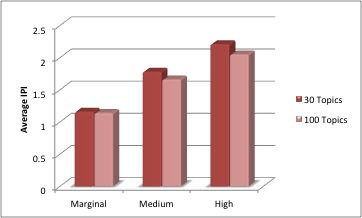
\includegraphics[scale=0.75]{IPIChart}
\end{center}
%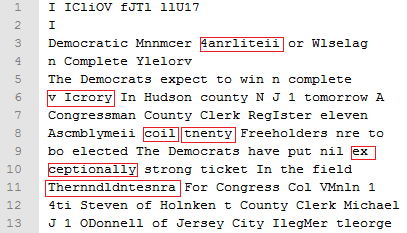
\includegraphics[scale=0.80]{ocr}
\caption{Comparison of the Average IPI for two ranked lists $L_1$ and $L_2$ using $30$ and $100$ topics respectively.}
\label{figure:IPI}
\end{figure*}

